\section{Game Theory Applications of EVIs}
\label{sec:games}

A major motivation for studying $\Phi$-EVIs lies in a strong connection to \emph{(C)CEs}~\citep{Aumann74:Subjectivity} in games. Indeed, we begin this section by pointing out that $\Phi$-EVIs capture 
(C)CEs for specific choices of $\Phi$. %It is worth pointing out that Aumann's key justification for CE was that such equilibria adhere to Bayesian rationality, which carries over to $\Phi$-EVIs.

We will mostly consider $n$-player \emph{concave} games. Here, each player $i \in \range{n}$ selects a strategy $\vx_i \in \cX_i$ from some convex and compact set $\cX_i$, and its utility is given by $u_i : (\vx_1, \dots, \vx_n) \mapsto \R$. We assume that $u_i(\vx_i, \vx_{-i})$ is differentiable and concave in $\vx_i$ for any $\vx_{-i}$, and that the gradients $\grad_{\vx_i} u_i(\vx_i, \vx_{-i})$ are bounded. We let $\cX \defeq \cX_1 \times \dots \times \cX_n$.

\begin{example}[CCE]
    \label{example:CCE}
    A distribution $\mu \in \Delta(\cX)$, is an \emph{$\epsilon$-coarse correlated equilibrium (CCE)}~\citep{Moulin78:Strategically} if for any player $i \in \range{n}$,
    \begin{equation}
        \label{eq:CCE-dev}
        \delta_i \defeq  \max_{\vx_i' \in \cX_i} \E_{\vx \sim \mu} u_i(\vx_i', \vx_{-i})  - \E_{\vx \sim \mu} u_i(\vx) \leq  \epsilon.
    \end{equation}
    Now, consider an $\epsilon$-approximate EVI solution $\mu$ of the problem defined by 
    $$F \defeq ( - \nabla_{\vx_1} u_1(\vx), \dots, - \nabla_{\vx_n} u_n(\vx)).$$ 
    Such $\mu$ satisfies, by concavity, $\sum_{i=1}^n \delta_i \leq \epsilon$; it is not necessarily an $\epsilon$-approximate CCE since it is possible that for some $i \in [n]$, {\em all} deviations strictly decrease $i$'s utility (so that $\delta_i$ in~\eqref{eq:CCE-dev} is negative)---$\mu$ is technically an \emph{average} CCE in the parlance of~\citet{Nadav10:Limits}. To capture CCE via $\Phi$-EVIs, one can instead consider a richer set of deviations of the form $(\vx_1, \dots, \vx_n) \mapsto (\vx_1, \dots, \vx_i', \dots, \vx_n)$ for all $i \in [n]$ and $\vx_i' \in \cX_i$.
\end{example}

A canonical example of the above formalism is a \emph{normal-form game}, in which each constraint set $\cX_i$ is the probability simplex $\Delta(\cA_i)$ over a finite set of \emph{actions} $\cA_i$, and each utility $u_i$ is a multilinear function.

\begin{example}[LCE]
    \label{example:CE}
    A distribution $\mu \in \Delta(\cX)$ is an \emph{$\epsilon$-linear correlated equilibrium (LCE)} if for any $i \in [n]$,
    \begin{equation*}
        \max_{\phi_i \in \Phi_i} \E_{ \vx \sim \mu } u_i(\phi_i(\vx_i), \vx_{-i}) - \E_{\vx \sim \mu} u_i(\vx) \leq \epsilon,
    \end{equation*}
    where $\Phi_i$ contains all linear functions from $\cX_i$ to $\cX_i$. To capture LCE via $\Phi$-EVIs, it suffices to consider deviations of the form $(\vx_1, \dots, \vx_n) \mapsto (\vx_1, \dots, \phi_i(\vx_i), \dots, \vx_n)$ for all $i \in [n]$ and $\phi_i \in \Phi_i$.
\end{example}

For normal-form games, LCEs amount to the usual notion of CEs~\citep{Aumann74:Subjectivity}. LCEs were introduced in the context of extensive-form games~\citep{Farina23:Polynomial,Farina24:Polynomial}.

\paragraph{Refining correlated equilibria} In fact, and more surprisingly, $\Philin$-EVI solutions can be a strict subset of LCEs.\footnote{The example of~\citet[Example 1]{Ahunbay25:First} already implies that certain CEs can be excluded from the set of $\Philin$-EVIs, which, incidentally, could have implications for last-iterate convergence in some classes of games, as discussed by that auhtor. Our example in~\Cref{fig:bach or stravinsky} goes much further, revealing that $\Philin$-EVIs can yield significantly different utilities for each player compared to CEs.} This separation can already be appreciated in the setting of normal-form games, and manifests itself in at least two distinct ways. First, there exist games for which a CE need not be a solution to the $\Philin$-EVI. In this sense, $\Philin$-EVIs yield a computationally tractable superset of Nash equilibria that is tighter than CEs. Second, computation suggests that the set of solutions of the $\Philin$-EVI for the game need not be a polyhedron, unlike the set of CEs. We provide a graphical depiction of this phenomenon in \cref{fig:bach or stravinsky}. The figure depicts the set of $\Philin$-EVI solutions to a simple ``Bach or Stravinsky'' game, in which the players receive payoffs $(3,2)$ if they both pick Bach, $(2,3)$ if they both pick Stravinsky, and $(0,0)$ otherwise.

\paragraph{Interpretation} The reason for this separation is that, for a map $\phi : \cX \to \cX$, each player's mapped strategy $\phi(\vx)_i$ can also depend (linearly) on {\em other players' strategies} $\vx_{-i}$. Indeed, the EVI formulation of a game does not take into account the identities of the players. For this reason, we will call the set of $\Philin$-EVI solutions in a concave game {\em anonymous linear correlated equilibria}, or {\em ALCE} for short. We give two game-theoretic interpretations of ALCEs.

First, the ALCEs of a game $\Gamma$ are the {\em symmetric} LCEs of the ``symmetrized'' game in which the players are randomly shuffled before the game begins. That is, consider the $n$-player game $\Gamma^\text{sym}$ defined as follows. Each player's strategy set is $\cX$. For strategy profile $(\vx^1, \dots, \vx^n) \in \cX^n$, the utility to player $i$ is given by 
\begin{equation*}
    u_i^\text{sym}(\vx^1, \dots, \vx^n) = \frac{1}{n!} \sum_{\sigma \in \Sym_n } u_{\sigma(i)}(\vx^{\sigma^{-1}(1)}_1, \dots, \vx^{\sigma^{-1}(n)}_n),
\end{equation*}
where $\Sym_n$ is the set of permutations $\sigma : [n] \to [n]$. The following result then follows almost by definition.
\begin{restatable}{proposition}{propJointLCESymmetric}\label{prop:joint lce symmetric}
    For a given distribution $\mu \in \Delta(\cX)$, define the distribution $\mu^n \in \Delta(\cX^n)$ by sampling $\vx\sim\mu$ and outputting $(\vx, \dots, \vx) \in \cX^n$. Then, $\mu$ is a ALCE of $\Gamma$ if and only if $\mu^n$ is an LCE of $\Gamma^\textup{sym}$. 
\end{restatable}

Second, for normal-form games, the ALCEs are the distributions $\mu \in \Delta(\cX)$ such that no player $i$ has a profitable deviation of the following form. The correlation device first samples $\vx\sim\mu$, and samples recommendations $a_j \sim \vx_j$ for each player $j$. Then, the player selects another player $j$ (possibly $j=i$) whose recommendation it wishes to see. The player then observes a sample $a_j' \sim \vx_j$ that is {\em independently} sampled from $a_j$.\footnote{This independence is crucial: without it, $\mu$ would actually need to be a distribution over pure Nash equilibria!} Finally, the player chooses an action $a_i^* \in \cA_i$, and each player $j$ gets reward $u_j(a_i^*, a_{-i})$. Thus, players are allowed (modulo the independent sampling) to {\em spy} on each others' recommendations.

Further discussion about ALCEs and formal proofs of the claims in this section are  deferred to \Cref{sec:appendix-joint}.

%Is it sufficiently clear that the operator is the game operator? I haven't checked. Ioannis: I can make it explicit in Example 5.1

% Insert here plot
\begin{figure}[t]
    \usepgfplotslibrary{fillbetween}
    \usetikzlibrary{patterns}
    \centering
    \scalebox{.8}{  
        \pgfplotsset{width=10cm,height=8cm,compat=1.18}
    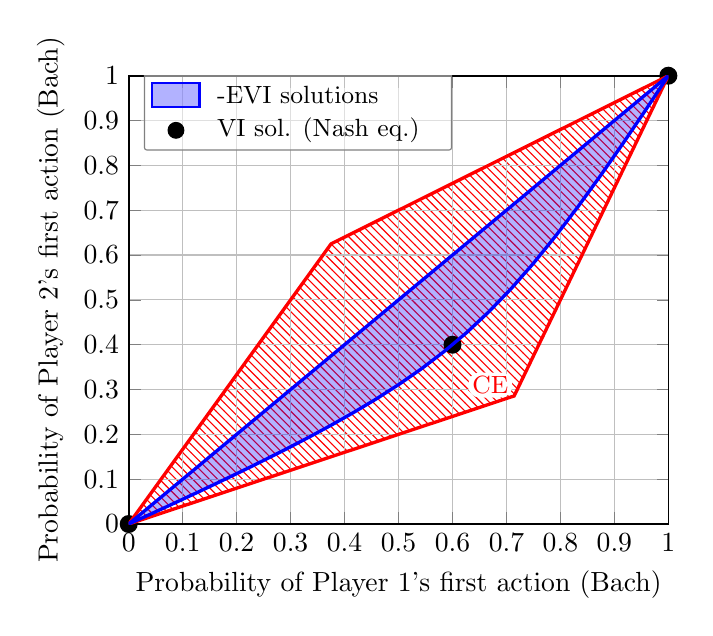
\begin{tikzpicture}
    \begin{axis}[grid,xmin=0,xmax=1,axis line style=semithick,xlabel={Probability of Player 1's first action (Bach)},ylabel={Probability of Player 2's first action (Bach)},ymin=0,ymax=1,xtick distance=0.1,ytick distance=0.1,clip marker paths=true,set layers,legend
    %, axis equal image
    ]
        \begin{pgfonlayer}{axis background}
            \fill [thick,pattern=north west lines,pattern color=red] (0,0) -- (0.7142857142760732, 0.28571428572392693) -- (1,1) -- (0.3750000001824576, 0.6249999998175428) -- cycle;
        \end{pgfonlayer}

        \draw [very thick,red] (0,0) -- (0.7142857142760732, 0.28571428572392693) -- (1,1) -- (0.3750000001824576, 0.6249999998175428)  -- cycle;

    
        \addplot [blue,very thick,name path=A,domain=0:1]
            {1/20 * (-11 + 25 * x + sqrt(121 - 310 * x + 225 * x^2))};
     
        \addplot [very thick, blue, name path=B,domain=0:1,samples=2]
            {x};
     
        \addplot [on layer=main,blue, fill opacity=0.3] fill between [of=A and B];
        % \fill [
        %     intersection segments={
        %         of=A and B,
        %         sequence=R1 -- L2},
        %     pattern=north east lines,
        % ] -- cycle;

        \begin{pgfonlayer}{pre main}
            \addplot[mark=*,only marks,mark size=1.0mm,thick] coordinates {(0,0) (.6,.4) (1,1)};
        \end{pgfonlayer}

        \node[red, inner sep=.5mm,rounded corners, fill=white,rotate=0] at (.67,.31) {\small CE};

        % \node[blue, inner sep=.5mm,rounded corners,rotate = 39] at (.5,.4) {\small \contour{white}{$\Philin$-EVI}};
        % \legend{CE,$\Philin$-EVI}

        \begin{scope}[x=1cm,y=1cm,yshift=5.2cm,xshift=2mm]
           \filldraw[gray,rounded corners=.3mm,fill=white,fill opacity=.5] (0,-.45) rectangle (3.9,1);
           \draw[thick,blue,fill=blue,fill opacity=.3] (.1,.1) rectangle (.7,.4);
           \node[anchor=west] at (.8,.25) {\small $\Philin$-EVI solutions};

           \draw[thick,red,pattern=north west lines,pattern color=red] (.1,.6) rectangle (.7,.9);
           \node[anchor=west] at (.8,.7) {\small Correlated equil.};

           \draw[fill=black] (.4, -.2) circle (1mm);
           % \draw[semithick] (.4, -.2) -- +(45:1mm) -- +(45:-1mm) -- (.4, -.2) -- +(135:1mm) -- +(-45:1mm);
           \node[anchor=west] at (.8,-.2) {\small VI sol. (Nash eq.)};
        \end{scope}
    \end{axis}
    \end{tikzpicture}}
    % \vspace{-2mm}
    \caption{
        Marginals of the set of correlated equilibria (CE) and of the set of solutions to $\Philin$-EVI in the simple $2 \times 2$ game ``Bach or Stravinsky.'' The x- and y-axes show the probability with which the two players select the first action (Bach). The set of marginals of $\Philin$-EVI solutions appears to have a curved boundary corresponding, we believe, to the hyperbola $10 x^2 - 25 xy + 10 y^2 - 6x+11y=0$.
    }
    \label{fig:bach or stravinsky}
    \vspace{-3mm}
\end{figure}

\paragraph{Coupled constraints}
Continuing from~\Cref{example:CCE,example:CE}, we observe that ($\Philin$-)EVIs can be used even in ``pseudo-games,'' in which $\cX$ does not necessarily decompose into $\cX_1 \times \dots \times \cX_n$; this means that $\vx_i \in \cX_i(\vx_{-i})$. As we discuss in~\Cref{sec:related}, most prior work in such settings has focused on generalized Nash equilibria, with the exception of~\citet{Bernasconi23:Constrained}. ($\Philin$-)EVIs induce an interesting notion of LCE/CCE in pseudo-games, albeit not directly comparable to the one put forward by~\citet{Bernasconi23:Constrained}. It is worth noting that~\citet{Bernasconi23:Constrained} left open whether efficient algorithms for computing their notion of (coarse) correlated equilibria exist.

\begin{definition}
    Given an $n$-player pseudo-game with concave, differentiable utilities and joint constraints $\cX$, a distribution $\mu \in \Delta(\cX)$ is an \emph{$\epsilon$-ALCE} if
    \begin{equation*}
        \max_{\phi \in \Philin} \E_{\vx \sim \mu} \sum_{i=1}^n u_i(\phi(\vx)_i, \vx_{-i}) - \sum_{i=1}^n u_i(\vx) \leq \epsilon.
    \end{equation*}
\end{definition}

By virtue of our main result (\Cref{th:elvi}), such an equilibrium can be computed in polynomial time.

\paragraph{Noncontinuous gradients} In fact, our results do not rest on the usual assumption that each player's gradient is a continuous function, thereby significantly expanding the scope of prior known results even in games. For example, we refer to~\citet{Dasgupta86:Existence,Bichler21:Learning,Martin24:Joint} for pointers to some applications.

\paragraph{Nonconcave games} Last but not least, $\Phi$-EVIs give rise to a notion of \emph{local} $\Phi$-equilibrium (\Cref{def:localPhi}) in nonconcave games. It turns out that this captures recent results by~\citet{Cai24:Tractable} and~\citet{Ahunbay25:First}, but our framework has certain important advantages. First, we give a $\poly(d, \log(1/\epsilon))$-time algorithm (\Cref{th:elvi}), while theirs scale polynomially in $1/\epsilon$. Second, our results do not assume continuity of the gradients. And finally, our algorithms are polynomial even when $\Phi$ contains all linear endomorphisms (\Cref{th:elvi}). \Cref{sec:localPhi} elaborates further on those points.